%\documentclass{article}
%\usepackage[T1]{fontenc}
%\usepackage[utf8]{inputenc}
%\usepackage{amsmath}
%\usepackage{amssymb}
%\usepackage{hyperref}
%\usepackage{parskip} %skip the indent of a new paragraph.
%\usepackage{float}
%\usepackage{graphicx}
%\usepackage{siunitx}
%\usepackage{listings}
%\usepackage{placeins}


\documentclass[pdftex,10pt,b5paper,twoside]{book}
\usepackage[lmargin=25mm,rmargin=25mm,tmargin=27mm,bmargin=30mm]{geometry}
\usepackage{caption}
\usepackage{subcaption}
\usepackage{cite}
\usepackage{amsmath,amssymb,amsfonts}
\usepackage{algorithmic}
\usepackage{graphicx}
\usepackage{textcomp}
\usepackage{gensymb}


\usepackage{setspace}
\usepackage{graphicx}
\usepackage{amssymb}
\usepackage{mathrsfs}
\usepackage{amsthm}
\usepackage{amsmath}
\usepackage{placeins}
%\usepackage[acronym]{glossaries}

% For side by side figures
%\usepackage{subfig}

% for multiline equations autosplit
%\usepackage{breqn}

%\usepackage[norsk]{babel}  % norske navn rundt omkring
%\usepackage[T1]{fontenc}   % norsk tegnsett (æøå)
%\usepackage[latin1]{inputenc} 

% Create argmin and argmax functions
\DeclareMathOperator*{\argmin}{argmin}   % Jan Hlavacek
\DeclareMathOperator*{\argmax}{argmax}   % Jan Hlavacek

\usepackage{color}
\usepackage[Lenny]{fncychap}
%\usepackage[pdftex,bookmarks=true]{hyperref}
\usepackage[pdftex]{hyperref}
%\usepackage{hyperref}
\hypersetup{
    colorlinks,%
    citecolor=black,%
    filecolor=black,%
    linkcolor=black,%
    urlcolor=black
}

\usepackage[font=small,labelfont=bf]{caption}
\usepackage{fancyhdr}
\usepackage{times}
\usepackage[acronym,toc]{glossaries}
\makeglossaries

% Trying to fix page number not showing up


% SI units and signs
\usepackage{siunitx}

% Write "Figures" instead of "List of Figures"
\renewcommand{\listfigurename}{Figures}

% Increase size of todos
%\setlength{\marginparwidth}{4cm}


%% Temporarily increase size of paper to add room for todos. REMEMBER TO REMOVE THIS FFS!
%\paperwidth=\dimexpr \paperwidth + 6cm\relax
%\oddsidemargin=\dimexpr\oddsidemargin + 3cm\relax
%\evensidemargin=\dimexpr\evensidemargin + 3cm\relax
%\marginparwidth=\dimexpr \marginparwidth + 3cm\relax



%\usepackage[intoc]{nomencl}
%\renewcommand{\nomname}{List of Abbreviations}
%\makenomenclature
\usepackage{natbib}
\usepackage{float}
\usepackage{parskip}
%\floatstyle{boxed} 
\restylefloat{figure}

% ShareLaTeX does not support glossaries now. Sorry...
%\usepackage[number=none]{glossary}
%\makeglossary
%\newglossarytype[abr]{abbr}{abt}{abl}
%\newglossarytype[alg]{acronyms}{acr}{acn}
%\newcommand{\abbrname}{Abbreviations} 
%\newcommand{\shortabbrname}{Abbreviations}
%%\makeabbr
%\newcommand{\HRule}{\rule{\linewidth}{0.5mm}}

\renewcommand*\contentsname{Table of Contents}

\pagestyle{fancy}
\fancyhf{}
\renewcommand{\chaptermark}[1]{\markboth{\chaptername\ \thechapter.\ #1}{}}
\renewcommand{\sectionmark}[1]{\markright{\thesection\ #1}}
\renewcommand{\headrulewidth}{0.1ex}
\renewcommand{\footrulewidth}{0.1ex}
%\fancypagestyle{plain}{\fancyhf{}\fancyfoot[LE,RO]{\thepage}\renewcommand{\headrulewidth}{0ex}}
\fancyfoot[C]{\thepage}
\newacronym{sintef}{SINTEF}{Selskapet for industriell og teknisk forskning ved Norges tekniske h\o gskole}
\newacronym{AD}{AD}{Actuaor disk}
\newacronym{WTM}{WTM}{Wind turbine model}
\newacronym{RWTM}{RTWM}{Rotating wind turbine model}
\newacronym{holes}{CH}{Circular Holes}
\newacronym{spider}{NU}{Non-Uniform}
\newacronym{PIV}{PIV}{Particle Image Velocimetry}
\glstoctrue

%\usepackage{cleveref}
\usepackage{todonotes}

\title{Development of a small-scale 
actuator disk}
\author{Sanne de Jong Helvig}
\date{2019}

\begin{document}

\begin{titlepage} % Suppresses displaying the page number on the title page and the subsequent page counts as page 1
	\newcommand{\HRule}{\rule{\linewidth}{0.5mm}} % Defines a new command for horizontal lines, change thickness here
	
	\center % Centre everything on the page
	
	%------------------------------------------------
	%	Headings
	%------------------------------------------------
	
	%\textsc{\LARGE Institution Name}\\[1.5cm] % Main heading such as the name of your university/college
	
	%\textsc{\Large Major Heading}\\[0.5cm] % Major heading such as course name
	
	%\textsc{\large Minor Heading}\\[0.5cm] % Minor heading such as course title
	
	%------------------------------------------------
	%	Title
	%------------------------------------------------
	
	\HRule\\[0.4cm]
	
	{\huge\bfseries 
	{\setstretch{1.0}
	Development of a small-scale actuator disk}\\[0.4cm] % Title of your document
	}
	
	\HRule\\[1.5cm]
	
	%------------------------------------------------
	%	Author(s)
	%------------------------------------------------
	
	\begin{minipage}{0.4\textwidth}
		\begin{flushleft}
			\large
			\textit{Author}\\
			\textsc{Sanne de Jong Helvig} % Your name
		\end{flushleft}
	\end{minipage}
	~
	\begin{minipage}{0.4\textwidth}
		\begin{flushright}
			\large
			\textit{Supervisor}\\
			\textsc{R. Jason Hearst}\\ % Supervisor's name
			%\textsc{Leif E. Andersson}\\ % Supervisor's name
			%\textsc{Konstanze K\"{o}lle} % Supervisor's name
		\end{flushright}
	\end{minipage}
	
	% If you don't want a supervisor, uncomment the two lines below and comment the code above
	%{\large\textit{Author}}\\
	%John \textsc{Smith} % Your name
	
	%------------------------------------------------
	%	Date
	%------------------------------------------------
	
	\vfill\vfill\vfill % Position the date 3/4 down the remaining page
	
	{\large\today} % Date, change the \today to a set date if you want to be precise
	
	%------------------------------------------------
	%	Logo
	%------------------------------------------------
	
	\vfill\vfill
	\includegraphics[width=0.6\textwidth]{0_Images/logontnu.pdf}\\[1cm] % Include a department/university logo - this will require the graphicx package
	 
	%----------------------------------------------------------------------------------------
	
	\vfill % Push the date up 1/4 of the remaining page
	
\end{titlepage}
\let\cleardoublepage\clearpage
%----------------------------------------------------------------------------------------


%\section*{Table of contents} 
\tableofcontents
\listoffigures
\printglossary[type=\acronymtype, title=List of Acronyms, toctitle=List of Acronyms]
\thispagestyle{empty} %Avoid page numbering on the table of contents
\newpage    

\setcounter{page}{1}
\let\cleardoublepage\clearpage
\chapter*{Abstract}
In this thesis, the drag of a small-scale rotating wind turbine model is measured in a wind tunnel. Actuator disks, with three different solidities and two different layouts, were designed and 3D printed. Then, the drag on the ADs was measured, and the results compared to the rotating wind turbine models in order to find the best match. The disk with a non-uniform design and a solidity of 35\% turned out to be the closest match. 

%should be in norwegian too 
%difference between abstract and conclusion... 

%less than 200-300 words, shorter than conclusion , con should cover every important finding 
%add acknowledgement
%can have citations in conclusion but not abstract %avoid acronyms in both 

%transducer and human error 
%reviewpapers!! %antonia pp compare, see dynamic differences 
%disks are based on this... 

%picture of PIV setup 
%in conclu, some problems, I learned did, created these curves, and these are the closest ones to go fort with 
\let\cleardoublepage\clearpage

\let\cleardoublepage\clearpage
\chapter*{Acknowledgements}
Firstly, I would like to thank my supervisor Jason, for always helping me out and supporting me. 

Magnus 

Olav, and crew 

Adi 

\let\cleardoublepage\clearpage
\chapter{Introduction}
In a world with a growing population, growing standards of living, and with it, a growing need for energy, simultaneous with an increasing focus on sustainability and environmentally friendly solutions, renewable energy has never been more relevant. The amount of onshore and offshore wind power is increasing, and numerous companies are working to find their role in the new market. Optimizing wind turbines and wind farms is an important aim, and researchers are using both simulations and experimental methods in order to explore different potentially efficient solutions. 

However, within both methods, modeling a wind farm with moving blades is often extremely complicated. Thus, simplifications, such as the actuator disk, are commonly adopted. The idea of the actuator disk is that it produces the same drag as the wind turbine, resulting in similar bulk characteristics in the wake. The physical wind tunnel analogue to an actuator disk is a static, porous disk. However, at this point in time, there are no clear directions and no scientific consensus on how to design and make these porous disks in order to mimic rotating turbines when conducting experiments.  


\section{Problem formulation}
The objective of the project described in this thesis is to develop a static, porous disk that has approximately matched characteristics to a small rotating wind turbine model provided by KTH, by matching the produced drag. In order to achieve this, the drag of the spinning wind turbine models are measured, and a variety of small-scale actuator disks are designed and 3D printed before drag measurements of the disks are conducted. Based on the results, the design will be honed in order to match the drag as closely as possible. 

%Eventuelt det om axial induction factor 

\let\cleardoublepage\clearpage
\chapter{Background}
Within the field of wind turbine aerodynamics, the actuator disk theory describes the simplest way to model a rotating turbine. The actuator disk is a non-rotating disk, physically modeled as a static porous disk. The idea is that the actuator disk produces the same drag as a moving turbine, resulting in the same bulk characteristics in the wake. 

The drag on the wind turbine models is the force in the direction parallel to the direction of the wind. The drag coefficient is further defined as 

\begin{equation}
    C_d = \frac{D}{\frac{1}{2}*\rho*u^2*A}
    \label{Eq:Cd}
\end{equation}

where $\rho$ is density, $u$ is the flow velocity and $A$ is the reference area.  

The drag on an object changes as the velocity changes. According to theory, $C_d$ increases as Re increases and then $C_d$ levels of at $ Re \simeq 10^3$, after which it remains approximately constant within the boundary of laminar flow. So this is the typical profile to expect when conducting drag measurements with varying Re. Here, Reynolds number is defined as 

\begin{equation}
    Re = \frac{\rho * u * L}{\mu}
\end{equation}

where $\rho$ is density, $u$ is velocity, $L$ is characteristic length and $\mu$ is the dynamic viscosity. For Reynolds number lower than $\simeq 5 * 10^5$ the flow is laminar, which is the type of flow relevant for this project. 






The porosity is a measure of the permeable area of the disc and is defines as the ratio between the open area and the total area of the disc. 


%Part 1, Why focus on wind? Why is this important and useful? 
%KAN NEVNA FNS MÅL 
Renewable energy now accounts for a third of global power capacity \cite{RenEnThirty}, and according to Siemens, wind power alone may represent one third of the of the global electric demand by 2040 \cite{WindThirty}. However, to realize these types of targets, larger wind farms covering increasingly larger surface areas are required \cite{Meyers2012} \cite{Stevens2017}. Placing the turbines in wind farms is namely the most economic and efficient in terms of planning, maintenance, and use of land and infrastructure \cite{Neunaber}. However, this means that the turbines are permanently exposed to the turbulent wakes caused by upstream rows of turbines \cite{Tossas2014}. Additionally, current utility-scale turbines extend a significant distance into the \gls{abl}, which is naturally turbulent \cite{Neunaber} \cite{Tossas2014}. 

The wake deriving from upstream wind turbines determine how much power a downstream turbine can generate and which mechanical loads it experiences, meaning that the study and characterization of wind turbine wakes has become an important research area \cite{Neunaber} \cite{Tossas2014}. According to a review paper by Veers et al (2019) \cite{Veers2019}, the first grand challenge in wind energy research today is improved understanding of wind power plant flow physics. According to another review by Porté-Agel et al (2019) \cite{PorteAgel2019}, there is a need for further investigating and developing models for win-farm wake flows and the role of atmospheric turbulence, as well as to extend wind farm studies to include factors such as topography and thermal stability. 

Variability in the power output due to unsteady characteristics of the \gls{abl} is another challenge for the integration of large amounts of wind energy intro the electricity grid, and the need for fill-in power and stronger components made to withstand unsteady loading turns the problem into that of a cost-minimizing problem, in order for wind energy to achieve the desired market share \cite{Bossuyt2016}. 

Studies of the interaction of large wind farms and the \gls{abl}, and how the wake develops and interacts with downstream wind turbine arrays, are currently not prevailing, and improved understanding of these phenomena is needed in order for wind farm developers to plan better-performing, less maintenance-intensive and longer-lasting wind farms, and for manufacturers to create better fatigue load-mitigating designs \cite{Tossas2014} \cite{Aubrun2019}. 


Field tests are being carried out, but such approaches are expensive, difficult and by their nature incapable of being completely controlled \cite{Sforza1981}. Even though there is a need for increased amounts of data from actual wind farms to evaluate experimental results, wind tunnel experiments have the advantage that the boundary conditions can be carefully controlled \cite{Bossuyt2016}. A challenge for studying wind farms in wind tunnels is performing measurements with sufficiently high spatial resolution, which has made small-scale turbines relevant, combined with the reduced costs \cite{Harrison2010} related to smaller models. The experts workshop organized by ForWind-Uni Oldenburg in 2018 on Wind Energy Science \& Wind Tunnel Experiments agreed to qualify the smallest wind turbine models, with a rotor diameter less than 0.5 m, as \gls{WGTM} \cite{Aubrun2019}.

However, using rotating blades for such small rotors, and building and operating more than a hundred of them, is not practical, but rather complex and costly. In addition, scaled rotating wind turbine models have limitations since prefect flow similarity is not possible due to large scale differences \cite{Bossuyt2016}. Thus, it is often convenient to use simplifications, a common one being the \gls{AD} concept. The physical representation of an \gls{AD} is a static, porous disk, with a solidity defined as 

\begin{equation}
    Solidity = \frac{}{}.
\end{equation}

Such porous disks work as a drag source and do not directly extract energy from the flow, in contrast to actual wind turbines, but instead dissipate the kinetic energy of the incoming wind by generating small-scale turbulence in the near wake of the disk \cite{Lignarolo2016}. 


\section{Actuator disk research}

Many researcher have looked into the actuator disk, most studying the disk in itself and comparing it to rotating models \cite{Lignarolo2014} \cite{Blackmore2013} \cite{Pierella2010} \cite{Aubrun2019} \cite{Cannon1993}  \cite{Sforza1981} \cite{Neunaber} \cite{Aubrun2013}, however some has gone so far as to use \gls{AD}s to model wind farms \cite{Bossuyt2016} \cite{Theunissen2014} \cite{Theunissen2018}. 

The first requirement for a simplified wind turbine model is correct characterization of the wake \cite{Theunissen2014}. When creating an \gls{AD}, the starting point is often to match the diameter and the drag coefficient, defined as

\begin{equation}
    C_d = \frac{D}{\frac{1}{2}*\rho*u^2*A}
    \label{Eq:Cd}
\end{equation}

Studies have shown that the drag coefficient is only weakly dependent on Reynolds number \cite{Blackmore2013}. 

When comparing \gls{AD}s and \gls{RWTM}s, studies conducted so far has a general agreement on the following terms. The near wake differs between the two models, as the rotating turbines introduce rotational momentum, tip and hub vortices, and turbulence from the blades, while the turbulence in terms of the \gls{AD} is produced by a grid \cite{Zhang2012} \cite{Lignarolo2014} \cite{Barthelmie2009}. The difference in flow behavior in the near wake, especially prominent in terms of velocity deficit and turbulence intensity, is thus caused by fundamentally different turbulence production and mixing mechanisms \cite{Aubrun2019} \cite{Lignarolo2016} \cite{Barthelmie2010}.

However, blade signatures and rotational momentum have shown to be overshadowed by ambient velocity fluctuations in the far wake \cite{Aubrun2013}. Thus, \gls{AD}s can create similar far wakes as rotating models, making them an appropriate substitution in the far wake, typically from $x/D = 3-4$, both at low and high inflow turbulence \cite{Lignarolo2014} \cite{Aubrun2013} \cite{Neunaber} \cite{Aubrun2019} \cite{Lignarolo2016}. Bossuyt et al (2016) \cite{Bossuyt2016} found that the disks are thus acceptable when studying wake interactions at wind farm scale.  

Despite the popularity of the simplifies model, few experimental studies are available. 









\section{Numerical use of actuator disks}

As mentioned, wind turbines are large, on the order of hundreds of meters, with a typical spacing within a wind farm of 5-10D, and a thickness of the blade on the order on 1 \si{m}. In order to resolve the full turbine geometry, ideally one would need to build a mesh with millimeter resolution around the blades inside a kilometer-scale computational box within the entire wind farm fits. As a consequence, simplifications are also used in \gls{CFD}. Many codes are based around the \gls{AD} concept, leading to many researchers working with simulations based \gls{AD}s \cite{Harrison2010} \cite{Tossas2014} \cite{Lignarolo2016} \cite{Wu2011} \cite{Wu2012} \cite{Simisiroglou2017} \cite{Stevens2014} \cite{StevensAlso2014}. Such modeling required fewer grid cells and not as small dimensions, allowing larger time steps. However, this efficiency comes at the expense of resolving the fine details of the blade boundary layers. If the objective is to study the far wake, this trade off is reasonable and using \gls{AD}s is more than acceptable. Work is being done in developing these models and comparing them to experimental results \cite{Harrison2010} \cite{Tossas2014}, including a organized workshop to compare different state-of-the-art numerical models for the simulation of wind turbine wakes \cite{LignaroloWorkshop2016}. With further development, a relatively inexpensive tool for the assessment of flow fields and planning of wind farms would be at hand for the industry \cite{Harrison2010} \cite{Sforza1981}. 

\section{Developing the actuator disk}

One main issue remains, as there is no standard for designing and making the \gls{AD}s today. Camp and Cal \cite{Camp2016} \cite{Camp2019} used a symmetric design, with a solidity that decreases with radial direction. Bossuyt et al (2016) \cite{Bossuyt2016} used a similar design, as well as Neunaber \cite{Neunaber}, who cut her disks from an aluminum plate. Aubrun et al \cite{Aubrun2013} used fine metal meshes with varying porosity at the center of the disc and at the outer edge. Later,Lignarolo et al (2016) \cite{Lignarolo2016} used a layered fine metal mesh. Blackmore et al (2013) \cite{Blackmore2013} used a pattern of circular, equally-sized holes to maintain approximately uniform porosity across the radius.  Sforza et al (1981) \cite{Sforza1981} used perforated metal plates, while Pierella and Sætran \cite{Pierella2010} used wooden grids. Myers et al (2010) \cite{Myers2010} used PVC plastic for their discs. In a round-robin conducted in 2019, both a metallic mesh with uniform porosity and a porous disc of plywood with radially non-uniform porosity was tested \cite{Aubrun2019}. Even though the simulated turbine will vary, and thus the diameter, porosity and drag coefficient of the \gls{AD}, a standard design creating the desired wake would be practical in order to create uniformity and comparability between experiments, and to save time so that every researcher around the world does not need to start the phase by developing their own disk. 


Theunissen et al (2014) \cite{Thenissen2014} used several different layouts, combining circular holes of different sizes as well as elongated bended fractures. Theunissen et al (2018) \cite{Theunissen2019} used circular, equally-sized holes, testing different topologies with the same porosity. 


%The wind turbines will grow in size, capacity and in terms of money invested \cite{Barthelmie2010}. 
%Wind energy will probably be an important contributor to production of affordable and clean energy in the next decades, 

%Current utility-scale turbines extend a significant distance into the atmospheric boundary layer, which is naturally turbulent \cite{Neunaber} \cite{Tossas2014}. 
%Further, placing the turbines in wind farms is the most economic and and efficient when it comes to planning, use of land and infrastructure, and maintenance \cite{Neunaber}. 

%Thus, wind turbines are permanently exposed to turbulence, either within the wind or when downstream turbines are hit by the turbulent wake created by upstream rows of turbines and their rotating turbine blades \cite{Neunaber} \cite{Tossas2014}. 

%Within a wind farm, as kinetic energy has been extracted from the wind and converted into electricity, the wind speeds do not recover to their freestream value after encountering the first row of turbines, and thus the wind speeds hitting subsequent turbines are lower than the freestream value \cite{Barthelmie2010}. Thus, the wake from the upstream wind turbines determine how much power a downstream turbine can generate and which mechanical loads it experiences, meaning that the study and characterization of wind turbine wakes has become an important research area. \cite{Neunaber} \cite{Tossas2014} When turbine spacing and wind farm layouts are considered in a conventional approach, decisions are made based on the desire to limit the wake-induced fatigue loads on downstream turbines \cite{Meyers2012}. 

%Variability in power output from wind turbines due to unsteady characteristics of the ABL is a challenge for the integration of large amounts of wind energy into the electricity grid, and the need for fill-in power and stronger components made to withstand unsteady loading turns the problem into that of a cost-minimizing problem, in order for wind energy to achieve the desired market share \cite{Bossuyt2016}


%Studies of the interaction of large wind farms and the ABL, and how the wake develops and interacts with downstream WT arrays, are currently not prevalent, and improved knowledge and understanding of the interaction is necessary \cite{Meyers2012} \cite{Bossuyt2016} \cite{Sforza1981} \cite{Tossas2014} \cite{Aubrun2019}. With improved understanding of this type of flows, wind farm developers can plan better-performing, less maintenance-intensive and longer-lasting wind farms, and manufacturers could create better fatigue load-mitigating designs \cite{Tossas2014}. 

%Part 2, why not alternatives

%Field tests are being carried out, but such approaches are expensive, difficult and by their nature incapable of being completely controlled \cite{Sforza1981}. Wind tunnel measurements have the advantage over full-scale experiments that the inflow and boundary conditions can be carefully controlled, and thus they can bring additional insight. \cite{Bossuyt2016}. Additionally, a wide range of inflow conditions can be tested and the created wake can be studied \cite{Sforza1981}. However, it should be mentioned that there is a need for increased amounts of data from actual wind farms, to evaluate whether experimental results are representative for the actual case. 

%A challenge for studying wind farms in wind tunnels is performing measurements with sufficiently high temporal and spatial resolution for a turbine array containing a large number of model turbines \cite{Bossuyt2016}. Therefore, small-scale turbines are relevant for experiments, and allow for extensive flow mapping studies to be conducted without the requirement of constructing scale turbines or the cost associated with large experimental test facilities\cite{Harrison2010}. The experts workshop organized by ForWind-Uni Oldenburg in 2018 on Wind Energy Science \& Wind Tunnel Experiments agreed to qualify the smallest wind turbine models, with a rotor diameter less than 0.5 m, as wake-generating turbine models, independent on whether they are steady or rotating models \cite{Aubrun2019}.

%However, using rotating blades for such small rotors, and building and operating 100 of them in a wind tunnel is not practical, but rather complex and costly. In addition, scaled rotating wind turbine models have inherent limitations since perfect flow similarity is not possible due to large scale differences. \cite{Bossuyt2016}. Rotating wind turbines can be compared to porous media due to their significant amount of flow-through. The question remains whether and to what extend it is possible to use simplified, non-rotating turbine models \cite{Neunaber}. 

%Oart 3, Why AD 

%In order to study the wake, several numerical and physical modeling approaches are used. Some model the wind turbine with the simplest model, the AD concept, adding a drag source within the surface swept by the blades \cite{Aubrun2013}. Porous disks are momentum sinks that does not directly extract energy from the flow, but instead dissipated kinetic energy of the incoming wind by generating small-scale turbulence in the near wake of the disk \cite{Lignarolo2016}. The simple but efficient actuator disk may be used as a simple method for simulating horizontal axis turbines. 


%Experiments
Multiple experimental studies concerning ADs have already been conducted. Some are at the stage of developing the AD itself. 

For example, Pierella and Sætran (2010) \cite{Pierella2010} studied the flow behind two circular grids of equal diameter and porosity but different mesh geometry. They used a biplane mesh, which turned out to produce a non-axisymmetric wake, and a monoplane mesh, giving an axisymmetric wake. The two wakes had different characteristics and the disks had different drags.

Earlier this year, nine research teams organized a round-robin measurement campaign of the wake of two porous discs in a homogeneous and low turbulent flow, performing similar wake measurements in different wind tunnels. \cite{Aubrun2019} In general, results collapsed reasonably well across facilities. 

Researchers such as Cannon et al. (1993) \cite{Cannon1993} have studied the wakes behind porous disks of varying solidity.

Others have gone further, and are moving towards the stage of using the actuator disks as simplifications for wind turbine models. 

Bossuyt et al (2016) \cite{Bossuyt2016} used 100 porous disk models to model a wind farm in a wind tunnel at different layouts, in order to study power output variability and unsteady loading in a turbulent boundary layer.  

Also \cite{Myers2010} did analysis on the flow field around horizontal axis tidal turbines using mesh disks as rotor simulators. 

In 1981, Sforza et al \cite{Sforza1981} used porous disks to simulate the effect of a wind turbine in order to investigate the wake, using both experimental and numerical methods.
%They concluded that the agreement between theory and experiment is quite reasonable, and that relatively simple turbulent flow analyses may be used with some success in describing the flow. 

\cite{Neunaber} investigated and compared an actuator disc and a model wind turbine exposed ti differnt uniform turbulent inflows, investigating the most variables. In the far wake, the wakes of both are similar. The results are independent on the inflow conditions. Velocity and turbulence intensity was different in the near wake. 



%near and far wake 
A first requirement for a scaled wind turbine representation is a correct characterization of the wake structure (Theunisen et al 2015). When creating an AD to represent a WT, the starting point is often to match the diameter and the drag. 

Studies conducted so far has a general agreement on the following terms. The near wake differs between the two models, as the turbulence in terms of the AD is produced by a grid, while rotating turbines introduce rotational momentum, tip and hub vorticies and turbulence from the blades (Zhang 2012). The difference in flow behaviour close to the model, especially prominent in terms of velocity deficit and turbulence intensity, is thus caused by fundamentally different turbulence production and mixing mechanisms, and leads to improper reproduction of the near flow \cite{Aubrun2019}. 

However, blade signatures and rotational momentum have shown to be overshadowed by ambient velocity fluctuations in the far wake \cite{Aubrun2013}. Porous disc models can create similar far wake as rotating models, making AD an adequate and appropriate substitution both at low and high inflow turbulence, typically from x/D = 3-4 \cite{Neunaber} \cite{Aubrun2019} \cite{Aubrun2013} \cite{Lignarolo2014} \cite{Thenuissen} \cite{CampCal}. and thus the disks are acceptable when studying wake interactions at wind farm scale. Bossuyt et al 2016 concluded that the experimental setup of a model wind farm is able to capture the main trends in mean row power and unsteady loading, making it useful for layout optimization studies. 

Studies have found that the drag coefficient is only weakly dependent on Reynolds number, so it remains roughly constant for a range of wind tunnel velocities. However, there is a dependence, meaning predictions of drag force with low levels of turbulence may differ from drag force experienced when operating in highly turbulent flow \cite{Blackmore2013}.

%The wake of the disc in the far field is an adequate substitution of the wake of the turbine, typically from neunabe 
%However, these small models are appropriate to model far-wake properties, and acceptable when studying wake interactions at wind farm scale. \cite{Aubrun2019}
%Porous disk models can create a similar far wake as rotating models in case of turbulent inflow conditions(Lignarolo 2014a, Aubrun 2013, Theunissen 2015, Camp cal 2016) They produce a similar far wake to a real turbine. 
% Can the wake be modeled properly in the absence of the rotation-induced tip votices, which are an important trigger for turbulent mixing and wake recovery? 


 


\subsection{Experimentally}

Lignarolo et al 2016 \cite{Lignarolo2016} provided an experimental analysis of the near-wake turbulent flow of a wind turbine and a porous disc. finding similarities and differences. They concluded that even in the absence of turbulence, the results show a good match in many variables such as thrust and energy coefficient, velocity, pressure and enthalpi. However, the turbulence intensity and turbulent mixing varied. The results suggested the possibility to extend the use of AD in numerical simulations until the very near wake, provided that turbulent mixing is correctly represented. The underlying question is how much the near wake differs given similarity of dimension, axial force and extracted energy. The stronger fluctuations in the WT wake are due to the pressence of concentrated tip vortices. They found the turbulence intensity of WT to be 2-4 times larger than for the AD wake in the near wake. Physics governing the turbulent mixing in the two wakes are intrinsically different. even in the absence of inflow turbulence, the velocity fields in the wakes are very well comparable. Again, extend the use of AD in numerical simulations until the very near wake. 

\cite{Lignarolo2016} also compared earlier experiments, showind a consistent decreasing drag coefficient with increasing porosity. 

Also the other Lignarolo: \cite{Lignarolo2014} conducted an experiemtnal study focusing on the comparison between the wake of a turbine and an AD. WT wake caracterized by complex dynamics of tip vortex development and breakdown, and turbulent fluctuations. Wake of AD is instead characterized by isotropic random fluctuations. Looking into the limitations. 

It is know that AD misestimates the effects of flow turbulence, due to the absence of the blade flow and its tip-vortes development and breakdown (Barthelie 2007). The mixing process across the wake interface and ultimately the rate at which the wake recovers the flow momentum is incorrectly modelled. 

The far wake region is typically less affected by the presence of the rotating blades. 

Despite the popularity of the simplified numerical model, few experimental studies are available., which analyse the flow field in he wake of an AD \cite{Lignarolo2014}. Matching the diameter and thrust coeff, the two give rise to the same wake expansion. 


Blackmore et al \cite{Blackmore2013} used experiments to investigate the effects of turulence on the drag of solid discs and porous disc turbine simulators. 

Aubrun et al (2013) \cite{Aubrun2013} studied wind turbine wake properties, by comparing a non-rotating simplified WT, based on the AD concept, and a rotating model, to determine the limits of the simplified model to reproduce a realistic wake. Concluding that the wakes, in the modeled ABL, were indistinguishable after 3D downstream. (in relatively high turbulent inflow conditions. Discrepancies still exist at x/d = 3 in low turbulent inflow conditions, but are relatively minor.  So the simplified AD model seems to be usable to reproduce the far wake. 





%\subsection{Use in CFD simulations}

%Numerical simulations and experimental studies can compliment each other for a better understanding. 

%As mentioned, wind turbines are large, on the order of hundreds of meters, with a typical spacing within a farm of 5-10 D, and a thickness of the blade on the order of 1m. In order to resolve the full turbine geometry, ideally one would need to build a mesh with submilimeter resolution in the blade BL inside a kilometer-scale computational box within the entire farm fits. As a consequence, we use a simplification: a model with an accuracy that generates the correct velocity deficit and TI in the far wake while ensuring that it is not too computanionally demaning. Thus, most codes rely on AD. \cite{Tossas2014} \cite{LignaroloWorkshop2016} \cite{Harrison2010} Such models are an attractive alternative, as they require fewer grid cells and not as small grid dimensions, allowing larger time steps. This efficiency comes at the expense of resolving the fine details of the blade BL, but if the objective is the far wake, this trade off is reasonable and AD is more than acceptable. As with experiments, a porous disc with the same diameter that applies a similar thrust force upon the moving fluid as a set of rotating blades may be used, but turbulence structures shed from the disk vary compared to the rotor in the near wake. Thus, AD is well suited for full wind farm computations. And work is being done in developing these models and comparing them to experimental results \cite{Harrison2010} \cite{Tossas2014}, including a organized workshop to compare different state-of-the-art numerical models for the simulation of wind turbine wakes \cite{LignaroloWorkshop2016}, especially comparing wakes produced from simulations to those produced with experiments. 

%Also on the computational area, more work related to AD is needed. For example, \cite{Tossas2014} claims the need for implementing a model for the wind turbine towel and nacelle to assess their impact on the turbine performance and wake profile. 

%Obtaining both real and experimental data is necessary in order to develop simulation methods and check simulated observations and predictions against actual wake characteristics. Experiments also provide data for computational model validation and for comparison for future work. 


%However, with such further development, a relatively inexpensive tool for assesment of flowfields and planning of wind farms would be at hand for the industry  (to enable the industrial use of CFD), and the CFD AD could be an accurate and validated method for numerically modelling turbines \cite{Sforza1981} \cite{Harrison2010}. 




%\subsection{Developing the actuator disk}

%One main issue remains, as there is no standard for designing and making the experimental actuator discs. Bossuyt et al (2016) \cite{Bossuyt2016} used a symmetric design, with a solidity that decreases with radial direction. Lignarolo et al (2016) \cite{Lignarolo2016} used a layered fine metal mesh, considered as a grid turbulence generator, while Aubrun et al \cite{Aubrun2013} used fine metal meshes with varying porosity at the center of the disc and at the outer edge. Blackmore et al (2013) \cite{Blackmore2013} used a hole pattern to maintain approximately uniform porosity across the radius. Aubrun et al \cite{Aubrun2019} used both a metallic mesh with uniform porosity and a porous disc of plywood with radially non-uniform porosity. Sforza et al (1981) \cite{Sforza1981} used perforated metal plates, while Pierella and Sætran \cite{Pierella2010} used wooden grids. Myers et al (2010) \cite{Myers2010} used PVC plastic for their discs. Even though the simulated turbine will vary, and thus the diameter, porosity and drag coefficient of the disc, a standard design creating the desired wake would be practical to create uniformity and comparability between experiments, and to save time so that every researcher around the world does not need to start the phase by developing their own disk. 

%Neunaber \cite{Neunaber} cut her disk from an aluminium plate in a non-uniform matter. She also highlited that she had a 100\% blockage in the center, where the nacelle is located in the case of a turbine, and that blackage shoul vary linearly similar to a real turbine. 


%Another detail to take into consideration at this point is the wind-tunnel blockage efffects created by the turbine models which may affect the wake. Thus, it is desired for the discs to be small \cite{Sforza1981}. 

%Also wanted further work, as to explain why a smaller diameter porous disc resulted in lower drag coeff than the larger diameter disc with same porosity. \cite{Blackmore2013}

%Nevertheless, in a direct experimental comparison of turbulent flow in the near wake, a porous disk (with same dimention and axial force as a rotating turbine) is currently not available \cite{Lignarolo2016}. Main drivers are porosity, structural stiffness, wake-flow uniformity 















\chapter{Method}

In the following, the process of designing, creating and testing the actuator disks will be presented, as well as the experimental setup. 

Ikke homogen freestream men wall effects 
definer spatial axes og origo 
%rod generates 3D flow disturbance characterized by overall downwash fra round robin







%Hvor kommer designene fra? 
%Hvor kommer solidityen fra?


%MÅL: 
%diameter bunn: 1.4cm 
%bunn høyde: 0.3 cm 
%total høyde: 6.6 cm ca (6.5 - 6.7) 
%diameter totalt: 0.4 cm 
%diameter blader: 4.5cm 


%står hub height 6cm. Som kan stemma hvis man trekke fra bunnen og sie at den e 0.4cm som altså er midt på stanga! 

%tykkelse på disk blir ca 0,5 i think 

%tverrstangå: 0.3cm tykk og 2cm lang midt te midt, also 1,5 cm bakover 

%magnetsize: 10mm dim og tykkelse bittelitt over 2mm
\section{Experimental setup}
%INCLUDE
%rod generates 3D flow disturbance characterized by overall downwash from round robin
%not homogeneous freestream men wall effects 

In order to measure the drag on the \gls{RWTM} and the \gls{AD}s, a wind tunnel and a force plate is needed as part of the experimental setup. There was also the need to construct a test rig on which the models could be placed inside the wind tunnel. 

\subsection{Force plate, wind tunnel and associated equipment}
The wind tunnel being used is 1 \si{\metre} wide and a 0.5 m tall. It has a maximum velocity of 35 m/s. The turbulence intensity is unknown, however it will be found when doing \gls{PIV} measurements in future work. Equipment can be placed inside the wind tunnel by removing a glass window which is 75 cm wide and 35 cm tall. The wind velocity is changed by manually turning a wheel, that in turn changes the position of the valves next to the motor inside the tunnel. At the floor of the tunnel there is a small hole, making it possible to connect the item one is measuring forces on inside the tunnel to the load cell underneath the tunnel.  

%Since the wheel is turned manually, based on a registered voltage related to the placement of the valves, recreating the exact same wind velocity two times in a row is almost impossible, and thus there will be minor variations in the velocity between the different measurements.

Underneath the wind tunnel is a force plate of the type AMTI BP400600HF 1000, able to measure the force and moment components along the x-, y- and z-axes. The force plate has an accuracy of ...  

%Here, the x-axis is defined to be along the length of the wind tunnel, parallelly to the wind velocity. The y-axis is defined to go across the width of the tunnel, while the z-axis goes along the height of the tunnel. Further, the origin is defined to be at the tunnel floor, in the center of the tunnel, as seen in figure. 
%Drawing showing axes 

The drag measured by the load cell is sent as a voltage signal through an amplifier. Afterwards, it is sent through a low pass filter, with a cut-off frequency of 1000 Hz. The data was gathered and saved using LabView, and the signal was turned back into a force using the given relationship between voltage and newton. 
%check cutoff! 

Inside the tunnel there is a sensor measuring the temperature, and a pitot tube measuring the pressure. The signal from the pitot tube is used to quantify the wind velocity. 
% 

%which measures the pressure and is used to quantify the wind velocity,
A potential uncertainty related to the wind tunnel is the fact that the pitot tube is placed in the vertical center of the tunnel, about 4 m upstream of the \gls{WTM}s. Thus, the velocity measured is not necessarily the same as the velocity that hits the \gls{WTM}s, which are placed close to the floor of the tunnel. Due to the development of wall boundary layers, the velocity hitting the \gls{WTM}s is likely lower than the measured and registered velocity. 
% at y=0, z=0.25 m, $x \approx -4 m$.


\subsection{The rig} 
The test rig consisted of a magnetic steel bar of 0.5 \si{\m} stretching across the width of the wind tunnel, on top of an aluminum cylinder which connects the bar to an aluminum plate, that in turn can be strapped to the load cell underneath the wind tunnel. Thus, the aluminum cylinder went through the hole at the bottom of the wind tunnel, and then the rest of the hole was covered with tape. Careful consideration was taken when adding the tape, so that the aluminum cylinder did not touch anything, as that would affect the force measurements. 
 %The rig was connected to the force plate using bolts, in such a way that the

The bar was lifted about 1 cm above the ground floor of the wind tunnel. Initially, it was desired to have the steel bar be almost as long as the width of the wind tunnel, in order to avoid affecting the flow outside of what is already the boundary layer in the tunnel. Similarly, it was desired to have the hub of the turbines exactly in the vertical middle of the tunnel to avoid the boundary layers. However, this was not doable. The hole in the bottom of the wind tunnel was limited in size, which meant that the steel bar could only be connected to the load cell underneath the tunnel through one aluminum cylinder with a small diameter of about 2 cm, making the support less robust. The length of the metal bar had to be shortened, and the bar had to be brought closer to the tunnel floor, in order to avoid bending and flapping at the ends.






 %50mm boundary layer in the other thesis, previous measurements in wind tunnel but PIV will tell me exactly. 
\section{Wind turbine models}
The two-bladed rotating \gls{WTM}s are the property of KTH in Stockholm, and can be seen in figure \ref{fig:rwtm}. They have a diameter of 45 \si{\mm}, and a hub height of approximately 65 \si{\mm}. Magnets are incorporated into the bottom of the models. 
%ADD PICTURE 


\begin{figure} 
    \centering
    \includegraphics[width=0.5\textwidth]{0_Images/RWTM.jpg}    
    \caption{One of the rotating models.}
    \label{fig:rwtm}
\end{figure}

\FloatBarrier
\section{The actuator disks}
As mentioned, there is no standard way of designing \gls{AD}s. In this project, the plan was to create \gls{AD}s with multiple solidities, and a possible method would have been to create two \gls{AD}s that were connected and could be rotated relative to each other in order to change the solidity. However, this seemed hard to achieve at such small scales. Pierella et al. \cite{Pierella2010} used \gls{PIV} measurements, Pitot tube measurements and \gls{CFD} simulations to study the flow behind two circular grids of equal diameter and porosity, one being a monoplane mesh and the other being a biplane mesh. The results showed that the biplane disk produced a lower drag than the monoplane disk, and that the two induced different wakes. The monoplane disk incuded an axisymmetric wake, while the biplane disk induced a non-axisymmetric flow dominated by the presence of trailing vortices. Thus, these two cases are not directly comparable, and since the goal of this project was to develop an \gls{AD} that does not induce a rotational element onto the flow, the monoplane disk was chosen. 



%I addition, based on the results of Pierella et al. \cite{Pierella2010}, a monoplane and a biplane \gls{AD} made with the same diameter and porosity produce different drags and result in different wakes, the monoplane disk producing a symmetric wake while the biplane disk creates a non-symmetric wake.


%In addition, the author was skeptic to the method based on the results of Pierella et al (2010) \cite{Pierella2010}, showing that a monoplane and a biplane \gls{AD} made with the same diameter and porosity produced different drags, making the cases not comparable. Since making a monoplane disk is probably simpler and easier to recreate, this method was chosen. 
 

\subsection{Computer-aided design and 3D printing}
The \gls{AD}s, as well as their towers, were designed using SolidWorks. Cura was used to turn the designs into readable code for the 3D printers, and the parts were then printed using a printer of the type Ultimaker 2+. The material used was PLA.
%3D printing was chosen as it is  repeatable 

A significant limitation occurred during the design process. The 3D printers available could not print thinner than 0.4 \si{\mm}, meaning that each line in the disks had to be at least 0.4 \si{\mm}. However, printing lines of 0.4 \si{\mm} proved troublesome, and it was decided that all lines should be equal to or thicker than 0.5 \si{\mm}. This is significant given that the disks are in themselves of such small dimensions. So there turned out to be a limit to how porous the disks could be made. 

%In general, a concern when using 3D printers is the fact that the print is not a hundred percent equal to the design - small variations may occur, making the actuator disks with the same design slightly different from each other. These slight variations matter more when the overall size of the design is so small compared to a larger design, however, the variations are still so few and small that they are considered to have close to no effect on the solidity or in making the disks differ from each other. In comparison, other methods of making ADs may also lead to minor differences. 

\subsection{Design of the tower}
The tower was designed to have the exact same dimensions as the given \gls{RWTM}'s tower. Most importantly, it had a hub height of 65 \si{\mm}. Underneath the base a hole was made that could fit a cylindrical neodymium magnet with a diameter of 10 \si{\mm}, a height of 2.5 \si{\mm} and a holding strength of 0.9 \si{\kg}. The \gls{AD}s were made to be interchangeable, and the end of the tower where the \gls{AD}s would be connected was made slightly thinner in order to fit into the designated holes in the \gls{AD}s. Three towers were printed, and one of them can be seen in figure \ref{fig:towers}.

\begin{figure}
    \centering
    \includegraphics[width=0.5\textwidth]{0_Images/tower.jpg}    
    \caption[The 3D printed tower.]{The 3D printed tower.}
    \label{fig:towers}
\end{figure}


\subsection{Actuator disk design}
The \gls{AD}s were designed with a diameter of 45 \si{\mm}, to match the \gls{RWTM}s. In an effort to have the same volume of the \gls{AD} as the swept volume of the blades, the blade is pointed straight down, and its projection on the $z$$x$-plane is studied. The thickest part of the projected blade is measured to be 5 \si{\mm}, whilst the thinnest part has approximately zero width. The thickest part is at the blade tip while the thinnest part is at the hub. Approximating the area of the blades when seen from the side as a triangle with height equal to the radius of the blade and base length equal to 5 \si{\mm} gives an estimate of the swept area, which is rotated around the hub to give the swept volume. In order to approximate the area with an \gls{AD} of constant width, the width should be half the size of the thickest part of the blades, i.e. 2.5 \si{\mm}. This gives approximately the same volume of the \gls{AD} as the swept volume of the blades.    

%Looking at the blades of the rotating model from the side, the two points furthest away from each other were measured to be about 5 \si{\mm} apart. In order for the disks to be representative of the blades, the disks were designed with a thickness of 2.5 \si{\mm}, corresponding to half of this maximum distance. 

%The thickest is 5, the thinnest is zero. 
%The disks were 2.5 \si{\mm} thick.

Two different designs of \gls{AD}s were tested. The first has numerous equally-sized holes spread symmetrically around the center point of the disk, as seen in figure \ref{Fig:holes60} and \ref{Fig:holes40}. It is quite similar to the design of Blackmore et al.  \cite{Blackmore2013}. The design is also meant to be comparable to those \gls{AD} designs that consist of a thin metal grid, similar to a grid turbulence generator, as used by Aubrun et al. and Lignarolo et al. \cite{Aubrun2013, Lignarolo2016}. The disks with this design will be called \gls{holes} going forth. The second design is also symmetric around the center point, but this one has rectangular holes that vary in size with radial distance, increasing in size as the radial coordinate increases, as seen in figure \ref{Fig:spider60} and \ref{Fig:spider40}. Thus, the solidity decreases with radial coordinate, matching the characteristics of an actual wind turbine. This design was used by Camp and Cal \cite{Camp2016, Camp2019} and by Neunaber \cite{Neunaber}. This design will be called \gls{spider}. 
%(however filled in to avoid sharp corners)


\begin{figure} [h!]
    \centering
    \begin{subfigure}[b]{0.45\linewidth}
        \includegraphics[width=\textwidth]{0_Images/holes60.jpg}
        \caption{The \gls{holes} design.}
        \label{Fig:holes60}
    \end{subfigure}
    ~
    \begin{subfigure}[b]{0.45\linewidth}
        \includegraphics[width=\textwidth]{0_Images/spider60.jpg}
        \caption{The \gls{spider} design.}
        \label{Fig:spider60}
    \end{subfigure}
    \caption{Actuator disks with a solidity of 60\%.}
    \label{Fig:60Sol}
\end{figure}

\begin{figure} [h!]
    \centering
    \begin{subfigure}[b]{0.45\linewidth}
        \includegraphics[width=\textwidth]{0_Images/holes40.jpg}
        \caption{The \gls{holes} design.}
        \label{Fig:holes40}
    \end{subfigure}
    ~
    \begin{subfigure}[b]{0.45\linewidth}
        \includegraphics[width=\textwidth]{0_Images/spider40.jpg}
        \caption{The \gls{spider} design.}
        \label{Fig:spider40}
    \end{subfigure}
    \caption{Actuator disks with a solidity of 40\%.}
    \label{Fig:40Sol}
\end{figure}

For each of these configurations, two solidities were created as an initial trial. The chosen solidities were 60\% and 40\%. A solid disk was also made as a reference case. Three disks of each design and solidity were printed. 

Based on the resulting drag profiles from the initial round of testing, two sets of \gls{AD}s with a solidity of 35\% were designed and printed, which can be seen in figure \ref{Fig:holes35} and \ref{Fig:spider35}. The first was made based on the \gls{holes} design. Due to the mentioned limitations regarding the printing thickness, providing a solidity less than 39\% with this design proved problematic. Hence the design was slightly changed, allowing for the holes to also cover the edges of the \gls{AD}s. It was kept in mind that this results in a different disk circumference, and that this might result in a drag force that is not directly comparable to the drag of the previously tested disks with the \gls{holes} design. The second disk was made using the \gls{spider} design. 

\begin{figure} [h!]
    \centering
    \begin{subfigure}[b]{0.45\linewidth}
        \includegraphics[width=\textwidth]{0_Images/holes35.jpg}
        \caption{The \gls{holes} design.}
        \label{Fig:holes35}
    \end{subfigure}
    ~
    \begin{subfigure}[b]{0.45\linewidth}
        \includegraphics[width=\textwidth]{0_Images/spider35.jpg}
        \caption{The \gls{spider} design.}
        \label{Fig:spider35}
    \end{subfigure}
    \caption{Actuator disks with a solidity of 35\%.}
    \label{Fig:35Sol}
\end{figure}

Each disk was, as mentioned, made with a small hole in the center, used to connect the disks to the tower. When connecting the two, this hole was filled in by the end of the tower, and so it did not affect the solidity of the disk. This design resulted in a larger solidity in the center of the disks, which can be argued to represent the nacelle of a wind turbine. A disk connected to a tower can be seen in figure \ref{Fig:towerAndAD}. 
%during the tests in the wind tunnel,



\begin{figure}
    \centering
    \includegraphics[width=0.5\textwidth]{0_Images/baseAndAD.jpg}    
    \caption[The tower connected to an actuator disk.]{The 3D printed tower connected to the 3D printed NUD with 35\% solidity.}
    \label{Fig:towerAndAD}
\end{figure}


%was made as the designs with rectangular holes that vary in size with radial distance.  

%PICTURE OF DISKS AND TOWER 
%there was a limit to how low the solidity could get, and 
%unrelated
\section{Testing}
The rig was connected to the force plate using bolts, in such a way that the aluminium cylinder came up through the hole on the bottom of the tunnel. The rest of the hole was covered with thick tape. Careful consideration was taken when adding the tape, so that the aluminium cylinder did not touch anything, as that would affect the force measurements. 

Given that the size of the wind turbine models is quite small, the turbines were tested in the wind tunnel three at a time, to ensure that the drag would be of an order that the instruments were able to measure and of an order were slight changes in the design resulting in slight changes in drag would be noticeable. The turbines were placed with a distance of 4D between them along the steel bar. The same was the case for the actuator disks. %KILDE  

Even though the turbine models were magnetic, it proved problematic to make them stay in the same position, with the turbine perpendicular to the wind direction, as the wind velocity increased. Thus, the models were connected to the steel bar using small pieces of tape. The 3D printed towers were able to stay in the right position on the base by themselves, still they were taped to the base like the rotating turbine models, to make sure the cases were comparable. 

As the drag is the force of interest in this work, only the force in the x-direction is measured. The force was measured for five different wind velocities; ~5 m/s, ~7.5 m/s, ~10 m/s, ~12.5 m/s and ~15 m/s. This corresponds to Reynolds numbers all of the order $10^4$. Since the velocity was changed by manually turning a wheel, a slight difference in the velocities occured between the different measurements. 

The force plate drifted over time, as is often the case with force measuring equipment. To take this into consideration when measuring the forces, zero measurements were conducted before and after every measurement. A 20 second tare measurement was first conducted. The wind tunnel was then turned on, with the velocity initially set to about 1 m/s, and then turned up to the wanted value. A measurement lasting one minute was then conducted. The velocity was once again reduced to about 1 m/s, and the wind tunnel was shut off. After the wind tunnel had quiet down and there was close to no moving air inside, another 20 second tare measurement was conducted. When measuring, a sampling rate of 1000 samples per second was used. 

Besides measuring the drag on the rotating turbine models and on all the different sets of actuator disks, a measurement was also conducted measuring only the drag on the base and the towers, without having any disks connected to them. 

Define spacial axes! 

%Based on the resulting drag profiles, the designs and solidities were to be adjusted. The iterative prosedure goes on until an actuator disk that has the same drag as the wind turbine model is presented.  

\section{Calculations}

For each disk at each wind velocity, the data collected from the wind tunnel consisted of a time series of voltages corresponding to the measured force and the measured wind velocity, as well as the times for when the first zero measurement and the second zero measurement was conducted and when the 60 second measurement started. Using Matlab, this data was treated.

A linear drift of the force plate was assumed. Thus, using the two zero measurement values, a linear function approximating the drift was created. The part of this linear function corresponding to the 60 seconds where the force measurement was conducted, was extracted. For each measured force in the time series, the corresponding drift was subtracted. After, the average force over the time series was calculated, as well as the variance and standard deviation. 

In the same matter, the drift was subtracted and the average force was calculated for the measurements of only the base and the tower. This was done for each of the different wind velocities. These averages were then subtracted from the averages calculated earlier, so that the final drag force was the force only on the disks, excluding the towers and the base. 

Finally, this calculated drag was divided by three, so as to only consider the drag on one disk. This force was used in calculating the drag coefficient, as well as the total swiping area of the rotating turbine model, being $\pi r^2$. 

Another value collected from the measurements was the average temperature during the 60 seconds of measuring, used to decide on the appropriate value for the air density when calculating the drag coefficient. 

Removing the towers: 
\cite{Aubrun2019} concluded that the discrepancy in rod fixation and distance between wall and disc center can generate different wake downwasg that might explain differences. 
%\input{4_Method/6_Flow_field_measurements.tex}
%\input{4_Method/7_Design_modifications.tex}
\chapter{Results \& Discussion}
After conducting the measurements, profiles showing the drag coefficient as a function of the wind velocity could be created for each set of disks, as well as for the rotating WT models. In this section, the drag and drag coefficient profiles are presented and discussed, as well as the calculated average Cd and the standard deviations. In the end, the measurement noise is discussed. 




\section{Rotational WT model}

The first measurement conducted using three rotating WT models resulted in a drag coefficient that was relatively independent of wind velocity for four of the measured wind velocities, but with a significant deviation at 5 m/s. To investigate whether this deviation was due to a measurement error, a second measurement was conducted, this time using three new rotating WT models. This second measurement gave more of an expected result at 5 m/s, however showed a deviation at 15 m/s. Thus, a third measurement, once again with three new rotating WT models, was conducted. Finally, a fourth measurement was carried out, this time using the same models as during the third measurement. The resulting drag coefficients can be seen as a function of wind velocity in figure \ref{fig:RotationalCD}.

\begin{figure}[h!]
    \centering
    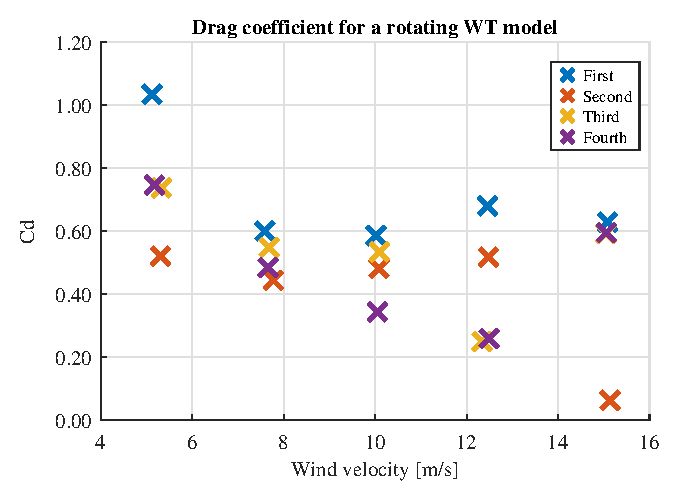
\includegraphics[width=\linewidth]{0_Images/RotationalCD.eps}
    \caption{The drag coefficient for the rotating WT models, obtained through four rounds of measurements.}
    \label{fig:RotationalCD}
\end{figure}

As can be seen, there is some variation between the different measurements. The values from the third and the fourth measurement, conducted using the same WT models, are quite similar at 5 m/s, 7.5 m/s and 12 m/s, and at 15 m/s, they completely overlap. This may show that the measurement is repeatable, and that one of the reasons for the varying results is simply that the rotating WT models have small differences, for example related to the friction of the rotating blades and how well they are connected. Be it too tight, there will be added friction. Be it too loose, the blades may start to oscillate. However, even between the third and fourth measurement, there is a noticeable difference at 7.5 m/s, showing that differences between the WT models is not the only cause for the varying results. 

Other possible causes of this variation may be related to noise and fluctuations in the applied wind velocity and in the force plate. 
%HOW CAN THIS BE EXPLAINED 

To investigate the results further, the drag resulting from the different measurements are pictured as a function of wind velocity in figure \ref{fig:RotationalDrag}


\begin{figure}[h!]
    \centering
    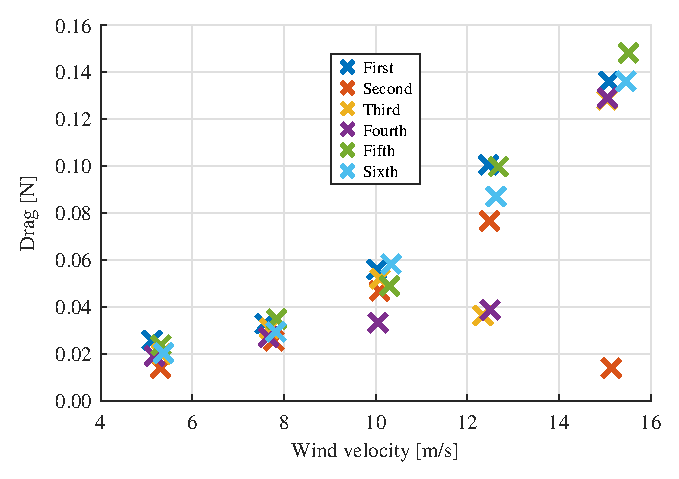
\includegraphics[width=\linewidth]{0_Images/RotationalDrag.eps}
    \caption{The measured drag for the rotating WT models, obtained through four rounds of measurements.}
    \label{fig:RotationalDrag}
\end{figure}

The drag at 12.5 m/s is lower than the drag at 10 m/s for the third measurement set, and the drag at 15 m/s is lower than the drag for 12.5 m/s for the second measurement set. This is not physical, and thus it is assumed that these two values are errors. The drag measured during the fourth measurement coincides with the disregarded drag from the third measurement, and is thus also regarded as an outlier. The wind tunnel did, for some unknown reason, seem to produce larger amounts of noise on the signal for velocities between 11 and 13 m/s, which might explain this repeated deviation. The drag at 10 m/s for the fourth measurement is higher than the drag at 7.5 m/s, however the value is lower than for all the measurements which seem to coincide quite well, and thus this value is considered as an outlier. The initial suspicious value, measured at 5 m/s in the first measurement, results in a $C_d$ larger than one, which seems unlikely, and hence this value is also regarded as an outlier. 
%AGREE? 

The outlier seem to be spread out both in terms of velocity at which they occur and in terms of whether they exceed or fall below the other values. One can argue that if taking a large number of new measurements, they would have a Gaussian distribution about a mean, and that taking the average of the values that seemingly coincide would be representative for this total mean. %Should probably be extended 

Thus, in order to achieve a representative value for the drag coefficient of the rotating WT models, the outliers were removed, and the average of the remaining drag coefficients was taken. This resulted in the drag coefficients seen in figure \ref{fig:RotationalAvg}.

\begin{figure}[h!]
    \centering
    \includegraphics[width=\linewidth]{0_Images/RotationalAverage.eps}
    \caption{The average drag coefficient for the rotational WT models for each wind velocity, based on the four conducted measurements, after removing the assumed wrongful outliers.}
    \label{fig:RotationalAvg}
\end{figure}

Assuming that $C_d$ is Reynolds number independent for such a short span at Reynolds numbers, the average over these measurement points is taken, resulting in an average $C_d$ of 0.585. Based on all the applied values, the standard deviation at hand is... Thus, when creating the ADs, this is the desired drag coefficient. 



\section{Drag on the ADs}
%kommenter at me uansett bryr oss mest om 10m/s, som e i den stabile delen 

The drag coefficient on the produced ADs has been studied. Initially, the solid disk, used as a reference case, produced the drag seen in figure \ref{Fig:SolidDrag} and the drag coefficient seen in figure \ref{Fig:SolidCD}. Further, the drag and the drag coefficient for the two types of disks with 60\% solidity can be seen in figure \ref{Fig:SixtyDrag} and \ref{Fig:SixtyCD}, respectively. For all three disks, the drag is seen to increase with increasing wind velocity, as one would expect. The average drag coefficient and the standard deviation is presented in table \ref{tab:AvgCD}.


\begin{figure} [h!]
    \centering
    \begin{subfigure}[b]{0.45\linewidth}
        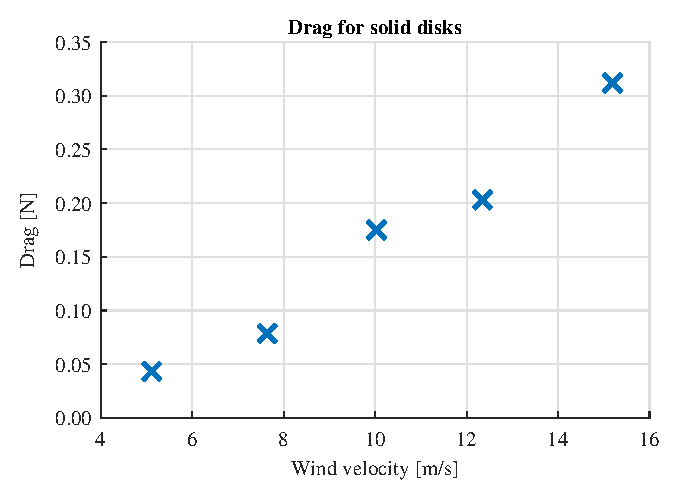
\includegraphics[width=\textwidth]{0_Images/SolidDrag.eps}
        \caption{The drag.}
        \label{Fig:SolidDrag}
    \end{subfigure}
    ~
    \begin{subfigure}[b]{0.45\linewidth}
        \includegraphics[width=\textwidth]{0_Images/SolidCD.eps}
        \caption{The drag coefficient.}
        \label{Fig:SolidCD}
    \end{subfigure}
    \caption{Using the solid disk.}
    \label{fig:SolidDisk}
\end{figure}


\begin{figure} [h!]
    \centering
    \begin{subfigure}[b]{0.45\linewidth}
        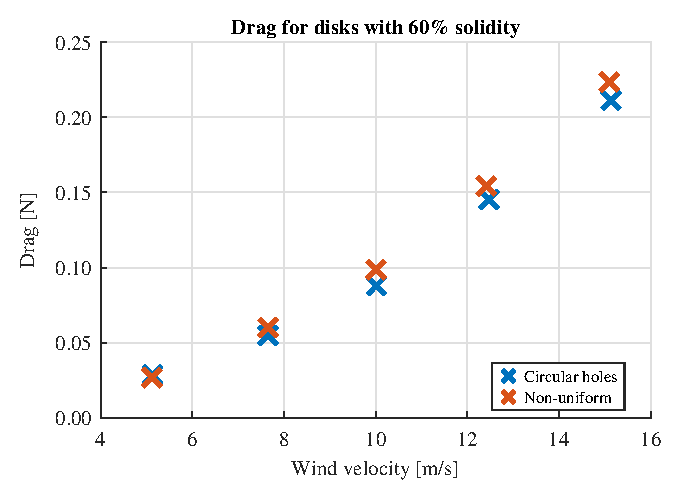
\includegraphics[width=\textwidth]{0_Images/SixtyDrag.eps}
        \caption{The drag.}
        \label{Fig:SixtyDrag}
    \end{subfigure}
    ~
    \begin{subfigure}[b]{0.45\linewidth}
        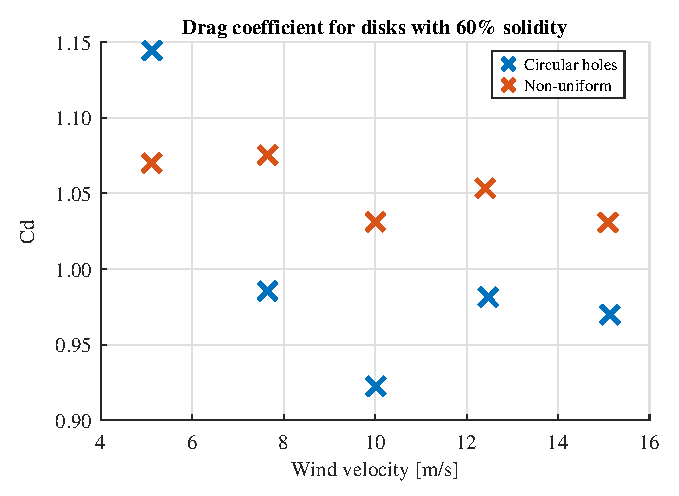
\includegraphics[width=\textwidth]{0_Images/SixtyCD.eps}
        \caption{The drag coefficient.}
        \label{Fig:SixtyCD}
    \end{subfigure}
    \caption{Using the disks with 60\% solidity.}
    \label{fig:SixtyDisk}
\end{figure}

\FloatBarrier

Further, the drag and drag coefficient for the disks with 40\% and 35\% solidity were plotted in figure \ref{fig:FortyDrag} and \ref{fig:FortyCD}. As these disks produced a drag coefficient fairly close to the average drag coefficient of the rotating turbines, this value is also included in the plots. The average drag coefficient and standard deviation can be seen in table \ref{tab:AvgCD}. 

\begin{figure}[h!]
    \centering
    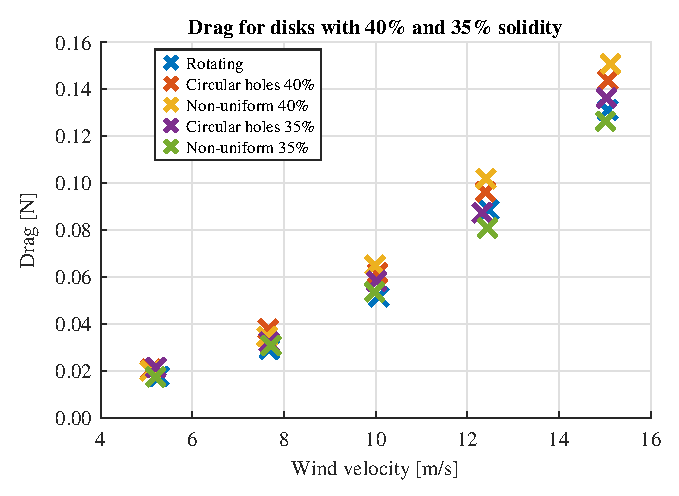
\includegraphics[width=\linewidth]{0_Images/FortyDrag.eps}
    \caption{The drag for the disks with 40\% and 35\% solidity, compared to the average drag coefficient of the rotating disks.}
    \label{fig:FortyDrag}
\end{figure}

\begin{figure}[h!]
    \centering
    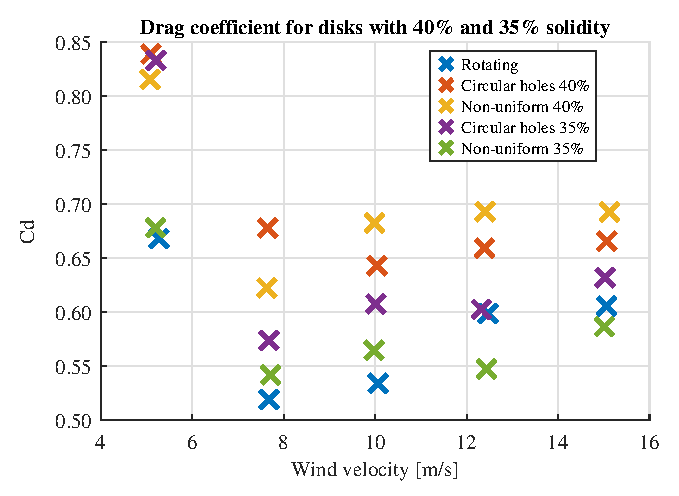
\includegraphics[width=\linewidth]{0_Images/FortyCD.eps}
    \caption{The drag coefficient for the disks with 40\% and 35\% solidity, compared to the average drag coefficient of the rotating disks.}
    \label{fig:FortyCD}
\end{figure}


Some general trends can be observed. For all disks presented in figure \ref{fig:FortyCD}, as well as for the disk with circular holes at 60\% solidity in figure \ref{Fig:SixtyCD}, Cd measured at 5 m/s is significantly higher than for the other velocities, while the measurements at the four other velocities seem to concentrate around some mean value. This may be a result of ... 


\begin{table}[H]
    \centering
    \begin{tabular}{l c c r}
         Disk type & Average Cd & SD \\
         \hline
         Rotating average & 0.5853 &  \\
         Solid & 1.5596 &  \\
         Uniform holes, 60\% & 1.0007 & \\
         Non-uniform, 60\% & 1.0521 &  \\
         Uniform holes, 40\% & 0.6970 &  \\
         Non-uniform, 40\% & 0.7013 &  \\
         Uniform holes, 35\% & 0.6499 & \\
         Non-uniform, 35\% & 0.5840 &  \\
    \end{tabular}
    \caption{Average Cd for each disk.}
    \label{tab:AvgCD}
\end{table}

%for last one, 0.5843 without drift 

In terms of these results, the non-uniform disk can be seen to produce a slightly higher drag at the same solidity compared to the uniform disk at 60\% and 40\% solidity. The same trend can not be seen at 35\% solidity, however this design with holes is created in a different way, with a larger circumference, and may not be exactly comparable. The non-uniform 35\% disk seems to best match the rotating WT model. 

As can readily be seen, the drag coefficient decreases with decreasing solidity, as one would expect. This can be compared to \cite{Lignarolo2016}, who presented a comparison between different drag coefficients as a function of solidity as presented in six different studies found in literature. According to this, a solidity of 60\% results in a Cd of around 0.9, a solidity of 40\% results in a Cd between 0.5 and 0.6, and a 35\% solidity results in a Cd between 0.4 and 0.5. Compared, the disks used in this study presents a higher drag for all solidities. This can be caused by conditions such as inflow turbulence. 

%Which SD is relevant? I have the ones for each measurement... But maybe the ones for Cd also? 

\section{Noise and other possible sources of error}

\begin{figure}[h!]
    \centering
    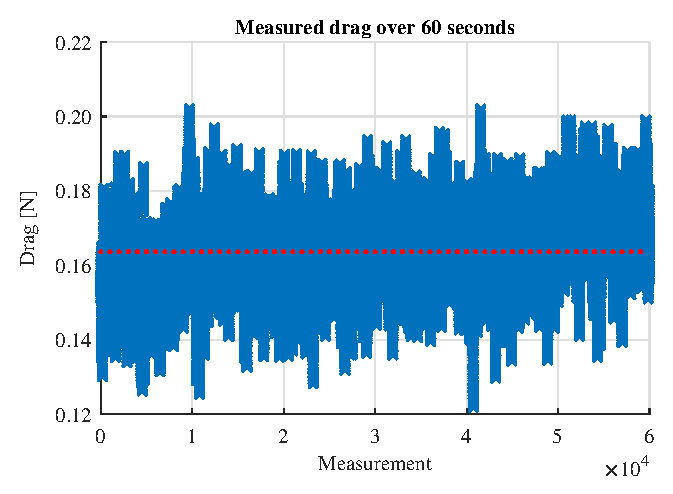
\includegraphics[width=\linewidth]{0_Images/NoiseFirst.eps}
    \caption{The drag for the solid disk at 5 m/s.}
    \label{fig:Noise}
\end{figure}

Figure \ref{fig:Noise} shows each measured drag value at a sampling rate of 1000 Hz over the course of 60 seconds. The measured drag varies with a 0.012, compared to an average of 0.1636. This means that the noise is of one order less that the average. 

This noise may both be related to measurement noise in the force plate, and electrical noise as the signal passes from the force plate, through the amplifier and the lowpass filter. It is still a reasonable assumption that the measurements have a Gaussian distribution and that the average drag is representative. 

The measured temperature only varies between about 20\degree C and 23\degree C. Since this variation is fairly small, it is assumed to not have any significant impact on the resulting drag. 



%Error, standard deviation 

%why do we get the results that we get? 

%- Adjusting for drift 
%- statistikk arument 
%- usikkerhet




%\section{Axial induction factor}

%\subsection{The wind turbine models}

%\subsection{The chosen actuator disk}

%\subsection{After further modifications}



\chapter{Future work}

A natural extension to this work would be to create more actuator disks, with solidities in between 35\% and 40\%, to see if it is possible to match the drag coefficient profile of the rotating turbine models even better.  

What I will do in my masters 


Future plans and outlook
Describe what you will do moving forward with this data for next term.  Maybe even propose a matrix of tests you intend to look at or write a little bit about the problems in the area you intend to investigate and how you will solve them.
\chapter{Conclusion}


In this thesis, an actuator disk that has a similar drag to a two-bladed rotating wind turbine model is found. The actuator disks were created using computer-aided design. Two different designs were testes, one with uniform holes inspired by the work of Aubrun et al (2013)\cite{Aubrun2013}, and one non-uniform design based on the disks used by Camp and Cal (2016)\cite{Camp2016}. The disks were made with three different solidities, 60\%, 40\% and 35\%. A solid disk was made as a reference case. All the disks had a hole in the center, used to connect them to the towers, thus making the disks interchangeable. The disks, as well as the towers, were 3D printed. 

Experiments were conducted using three models at the same time, to make sure the drag would be of an order were slight changes in solidity and the resulting changes in the drag would be noticeable by the force plate being used. Measurements were done for five different Reynolds numbers, all of the order $10^4$. Initial tests showed that the force plate drifted over time. To solve this, zero measurements were conducted before and after each measurement. A linear drift was assumed, and for each measurement, the corresponding drift was subtracted. Measurements were also conducted on only the towers and the base that the models were placed on inside the tunnel, so that this drag could be subtracted from the previous drag measurements, leaving only the drag on the disks and on the rotating blades.  

When conducting the measurements of the rotating models, some of the resulting drag coefficients deviated from the rest, however these deviations differed in size and appeared at different velocities. Thus, six different measurements were conducted, all using different sets of rotating models, except for two of them that used the same set. The reasons behind the deviations were concluded to be variations between the rotating models, noise in the transducer, and human error. It was solved by discarding those measurements regarded as outliers, and taking the average over the remaining drag coefficients at each velocity. This uncertainty related to the rotating models supports the claim that there is a need for alternative ways of modelling wind turbines. 
%some deviations in the resulting drag coefficient appeared, however differing in size and appearing at different velocities. 

The drag and drag coefficients deriving from all the different actuator disks were then studied. Some general trends showed that the drag increases with increasing Re, and that the drag coefficient increases with increasing solidity, as supported by literature \cite{Lignarolo2016}. Additionally, the drag coefficient seems to be Reynolds independent for four of the Reynolds numbers, but the drag coefficient at $Re \approx 1.5*10^4$ deviates from the others, most likely due to the increased sensitivity at such a low velocity and the impact of noise on such a small drag. Based on the average drag coefficient, the non-uniform disk with 35\% solidity seems to best match the rotating model, while the 35\% solidity disk with uniform holes is the second closest match. Assuming a Gaussian distribution of the drag coefficients, both of the disks with 35\% solidity had the rotating models drag coefficient within its standard deviation, showing that it is reasonable to use these actuator disks to mimic the rotating model. 

%Assuming that the drag coefficient from the rotating model is correct and assuming a Gaussian distribution of the drag coefficients for the actuator disks, both of the disks with 35\% solidity had the rotating models drag coefficient within its standard deviation, showing that it is reasonable to use these actuator disks to mimic the rotating model. 
%to measurement noise at such low drags.

In future work, the wakes of these two models will be studied using Particle Image Velocimetry, and compared to the wake of the rotating model, investigating factors such as velocity deficit, turbulence intensity and rotation of the flow. The models will also be used to simulate a wind farm, and similarities and differences between the resulting flow fields will be studied. 










%Conclusions
%Bring up the main points from the document, highlighting the method, results, conclusions, and where you will go next.  This will be the last thing the grader reads, so you really want to remind the reader of all the good work you did.

%Finn guidelines for vurdering av prosjektoppgave 




%bartheime og jensen, reduseres 20 prosent, derfor må vi finne ut om dette funker 
  
  
%The drag of a small-scale rotating wind turbine model was measured in a wind tunnel, and compared to the drag of different actuator disks, in order to find the actuator disk that most resembles the rotating model. The actuator disks were created with two different designs, one with uniform holes and one non-uniform, and three different solidities were used within each design. A solid actuator disk was also tested. The drag on the actuator disks were measured in the wind tunnel in the same matter as with the rotating model, using five different Reynolds numbers. When conducting the experiments, several measurements of the rotating models had to be conducted due to deviations in the measurement data. Some of these deviations were regarded as outliers and discarded, and the average was taken of the remaining measurements. This resulted in a drag coefficient profile which was compared to the drag coefficient profiles representing the different actuator disks. The disk with a non-uniform design and a solidity of 35\% turned out to be the closest match, while the disk with uniform holes and a solidity of 35\% was the second closest match. Assuming that the drag coefficient from the rotating model is correct and assuming a Gaussian distribution of the drag coefficients from the actuator disks, both of the disks with 35\% solidity had the rotating models drag coefficient within its standard deviation, showing that it is reasonable to use these actuator disks to mimic the rotating model. 





\newpage
%\addcontentsline{toc}{Chapter}{References} %uncomment if you want the references included in the table of content
%\bibliographystyle{plain}
\bibliographystyle{unsrt}
\bibliography{ref.bib}

%\addcontentsline{toc}{Chapter}{List of Acronyms}
%\printglossary[type=\acronymtype, title=List of Acronyms, toctitle=List of Acronyms]

\end{document}
